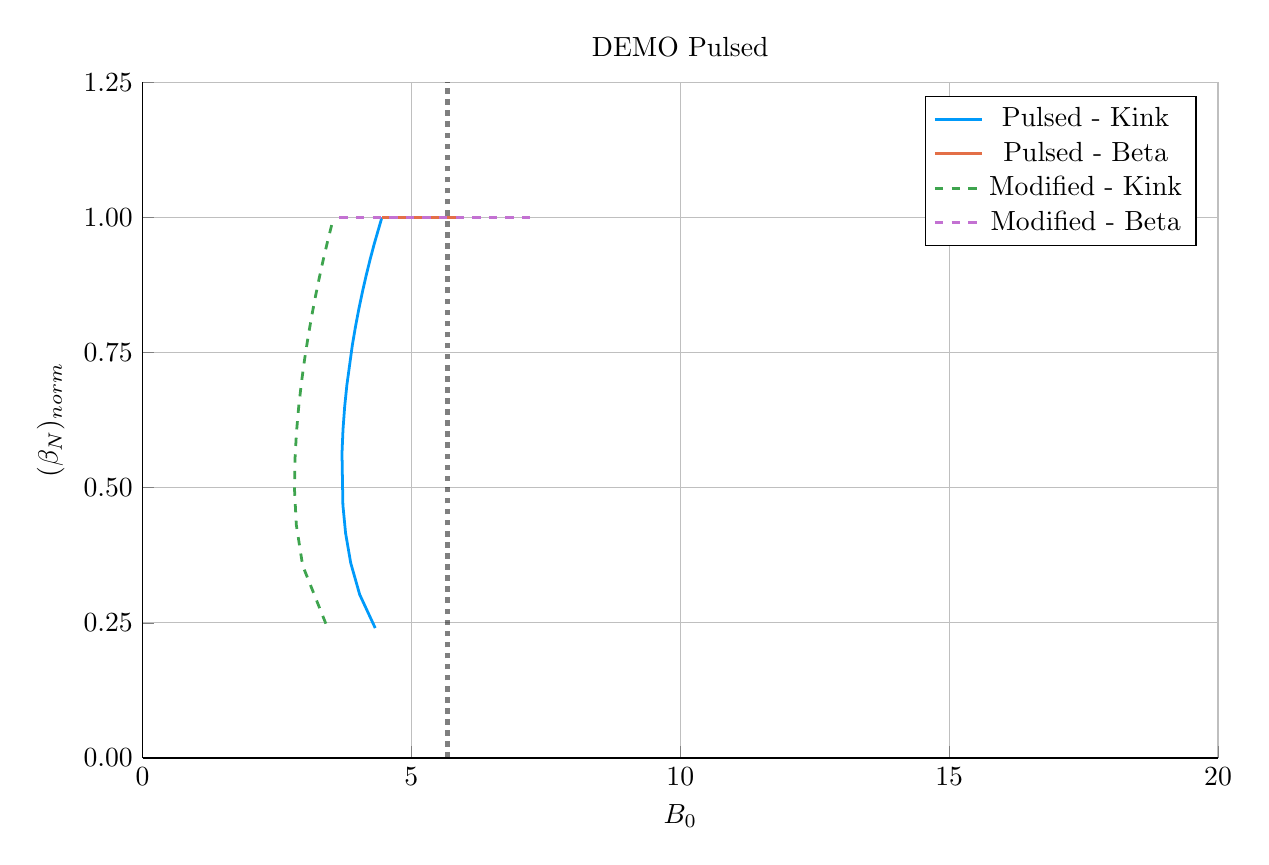
\begin{tikzpicture}[]
\begin{axis}[height = {101.6mm}, ylabel = {$( {\beta}_{N} )_{norm}$}, title = {DEMO Pulsed}, xmin = {0.0}, xmax = {20.0}, ymax = {1.25}, xlabel = {${B}_{0}$}, {unbounded coords=jump, scaled x ticks = false, xticklabel style={rotate = 0}, xmajorgrids = true, xtick = {0.0,5.0,10.0,15.0,20.0}, xticklabels = {0,5,10,15,20}, xtick align = inside, axis lines* = left, scaled y ticks = false, yticklabel style={rotate = 0}, ymajorgrids = true, ytick = {0.0,0.25,0.5,0.75,1.0,1.25}, yticklabels = {0.00,0.25,0.50,0.75,1.00,1.25}, ytick align = inside, axis lines* = left,     xshift = 0.0mm,
    yshift = 0.0mm,
    axis background/.style={fill={rgb,1:red,1.00000000;green,1.00000000;blue,1.00000000}}
, colorbar style={title=}}, ymin = {0.0}, width = {152.4mm}]\addplot+ [color = {rgb,1:red,0.00000000;green,0.60560316;blue,0.97868012},
draw opacity=1.0,
line width=1,
solid,mark = none,
mark size = 2.0,
mark options = {
    color = {rgb,1:red,0.00000000;green,0.00000000;blue,0.00000000}, draw opacity = 1.0,
    fill = {rgb,1:red,0.00000000;green,0.60560316;blue,0.97868012}, fill opacity = 1.0,
    line width = 1,
    rotate = 0,
    solid
}]coordinates {
(4.327031075670194, 0.2404246203728706)
(4.038214026054326, 0.3023615610883452)
(3.8713719163129245, 0.36084052767821884)
(3.7758613845615545, 0.41598982346603114)
(3.7257856761317214, 0.468022970395578)
(3.7090473695925437, 0.5636986930703128)
(3.727711597554826, 0.607802240159545)
(3.7586131667481433, 0.6496939342691259)
(3.799052518631718, 0.6895565401580928)
(3.901290136389271, 0.763829276228584)
(3.960577465316514, 0.7985141004724962)
(4.0241209645210345, 0.8317230980567779)
(4.0912717805663785, 0.8635594422549302)
(4.161514602943343, 0.8941156370979517)
(4.2344343960723005, 0.9234748795254103)
(4.309692554546368, 0.9517122356163621)
(4.450417240491067, 1.0000000000000007)
};
\addlegendentry{Pulsed - Kink}
\addplot+ [color = {rgb,1:red,0.88887350;green,0.43564919;blue,0.27812294},
draw opacity=1.0,
line width=1,
solid,mark = none,
mark size = 2.0,
mark options = {
    color = {rgb,1:red,0.00000000;green,0.00000000;blue,0.00000000}, draw opacity = 1.0,
    fill = {rgb,1:red,0.88887350;green,0.43564919;blue,0.27812294}, fill opacity = 1.0,
    line width = 1,
    rotate = 0,
    solid
}]coordinates {
(4.450417240491067, 1.0000000000000007)
(4.490148631384312, 1.0000000000000007)
(4.692490181445514, 1.0)
(4.8960344619053355, 1.0)
(5.100651132702229, 0.9999999999999989)
(5.306202822090688, 0.9999999999999994)
(5.512545696627038, 1.0)
(5.719530043226767, 1.0)
(5.927000883375481, 1.0000000000000009)
};
\addlegendentry{Pulsed - Beta}
\addplot+ [color = {rgb,1:red,0.24222430;green,0.64327509;blue,0.30444865},
draw opacity=1.0,
line width=1,
dashed,mark = none,
mark size = 2.0,
mark options = {
    color = {rgb,1:red,0.00000000;green,0.00000000;blue,0.00000000}, draw opacity = 1.0,
    fill = {rgb,1:red,0.24222430;green,0.64327509;blue,0.30444865}, fill opacity = 1.0,
    line width = 1,
    rotate = 0,
    solid
}]coordinates {
(3.4087424183072135, 0.248606549150966)
(2.977074181068944, 0.3560931641184958)
(2.8592500074202523, 0.4316291993785841)
(2.827199220063259, 0.49490432276768237)
(2.8339789008667826, 0.5511525448438662)
(2.862412302880871, 0.602602481926993)
(2.9044598258085443, 0.6504302545880215)
(2.95577893007882, 0.6953433668883134)
(3.0137895352525907, 0.7378079400968965)
(3.076849710218805, 0.7781526533692803)
(3.1438583711612704, 0.8166218695399752)
(3.214045733980633, 0.8534051004492762)
(3.2868548955983727, 0.8886544154056605)
(3.361871149981842, 0.9224952625580776)
(3.4387778750377818, 0.9550334859574554)
(3.5173279629378453, 0.9863600431607767)
};
\addlegendentry{Modified - Kink}
\addplot+ [color = {rgb,1:red,0.76444018;green,0.44411178;blue,0.82429754},
draw opacity=1.0,
line width=1,
dashed,mark = none,
mark size = 2.0,
mark options = {
    color = {rgb,1:red,0.00000000;green,0.00000000;blue,0.00000000}, draw opacity = 1.0,
    fill = {rgb,1:red,0.76444018;green,0.44411178;blue,0.82429754}, fill opacity = 1.0,
    line width = 1,
    rotate = 0,
    solid
}]coordinates {
(3.6607028750648505, 1.000000000000001)
(3.8574448036470477, 1.0000000000000002)
(4.056375867871351, 1.0000000000000002)
(4.257366397480293, 1.0000000000000009)
(4.460279103534801, 0.9999999999999996)
(4.664969389370631, 1.0)
(4.871285596007394, 1.0)
(5.07906923307514, 1.0000000000000002)
(5.288155233306219, 1.0)
(5.498372259673351, 0.9999999999999998)
(5.709543087166185, 1.0000000000000004)
(5.921485076209294, 1.0000000000000002)
(6.134010749367255, 1.000000000000001)
(6.346928478632384, 0.9999999999999996)
(6.560043285872518, 1.0)
(6.773157754368795, 1.0)
(6.986073044284746, 1.0000000000000002)
(7.198590001107076, 1.0000000000000002)
};
\addlegendentry{Modified - Beta}
\addplot+ [color = {rgb,1:red,0.00000000;green,0.00000000;blue,0.00000000},
draw opacity=0.5,
line width=2,
dotted,mark = none,
mark size = 2.0,
mark options = {
    color = {rgb,1:red,0.00000000;green,0.00000000;blue,0.00000000}, draw opacity = 0.5,
    fill = {rgb,1:red,0.00000000;green,0.00000000;blue,0.00000000}, fill opacity = 0.5,
    line width = 1,
    rotate = 0,
    solid
},forget plot]coordinates {
(0.0, NaN)
(20.0, NaN)
};
\addplot+ [color = {rgb,1:red,0.00000000;green,0.00000000;blue,0.00000000},
draw opacity=0.5,
line width=2,
dotted,mark = none,
mark size = 2.0,
mark options = {
    color = {rgb,1:red,0.00000000;green,0.00000000;blue,0.00000000}, draw opacity = 0.5,
    fill = {rgb,1:red,0.00000000;green,0.00000000;blue,0.00000000}, fill opacity = 0.5,
    line width = 1,
    rotate = 0,
    solid
},forget plot]coordinates {
(5.667, 0.0)
(5.667, 1.25)
};
\addplot+[draw=none, color = {rgb,1:red,0.00000000;green,0.00000000;blue,0.00000000},
draw opacity=0.5,
line width=0,
solid,mark = *,
mark size = 2.0,
mark options = {
    color = {rgb,1:red,0.00000000;green,0.00000000;blue,0.00000000}, draw opacity = 0.5,
    fill = {rgb,1:red,0.00000000;green,0.00000000;blue,0.00000000}, fill opacity = 0.5,
    line width = 1,
    rotate = 0,
    solid
},forget plot] coordinates {
(5.667, NaN)
};
\end{axis}

\end{tikzpicture}
